\documentclass{article}
\usepackage{amsmath}
\usepackage{tcolorbox}
\usepackage[margin=0.5in]{geometry} 
\usepackage{amsmath,amsthm,amssymb,amsfonts, fancyhdr, color, comment, graphicx, environ}
\usepackage{float}
\usepackage{xcolor}
\usepackage{mdframed}
\usepackage[shortlabels]{enumitem}
\usepackage{indentfirst}
\usepackage{mathrsfs}
\usepackage{hyperref}
\graphicspath{{./}{gr/}}
\makeatletter
\newcommand*{\rom}[1]{\expandafter\@slowromancap\romannumeral #1@}
\makeatother
% Change enumerate labels to (a), (b), (c), ...
% Define a new environment for problems
\newcounter{problemCounter}
\newtcolorbox{problem}[2][]{colback=white, colframe=black, boxrule=0.5mm, arc=4mm, auto outer arc, title={\ifstrempty{#1}{Problem \stepcounter{problemCounter}\theproblemCounter}{#1}}}

% \renewcommand{\labelenumi}{\alph{enumi})}
\def\zz{{\mathbb Z}}
\def\R{{\mathbb R}}
\def\qq{{\mathbb Q}}
\def\cc{{\mathbb C}}
\def\N{{\mathbb N}}
\def\ss{{\mathbb S}}

\newcommand{\p}{\partial}
\renewcommand{\vec}[1]{\mathbf{#1}}
\newcommand{\vx}{\vec{x}}
\newcommand{\Lag}{\mathcal{L}}
\newcommand{\sep}{\,:\,}


\newtheorem{theorem}{Theorem}[section]
\newtheorem{corollary}{Corollary}[theorem]
\newtheorem{lemma}[theorem]{Lemma}
\newtcolorbox{proposition}[1][]{colback=white, colframe=blue, boxrule=0.5mm, arc=4mm, auto outer arc, title={Proposition #1}}
\newtcolorbox{definition}[1][]{colback=white, colframe=violet, boxrule=0.5mm, arc=4mm, auto outer arc, title={Definition #1}}
\newcommand{\Zmod}[1]{\zz/#1\zz}
\newcommand{\partFrac}[2]{\frac{\partial #1}{\partial #2}}

\newcommand\Mydiv[2]{%
$\strut#1$\kern.25em\smash{\raise.3ex\hbox{$\big)$}}$\mkern-8mu
        \overline{\enspace\strut#2}$}

\begin{document}

\begin{center}
    Math 714
    \hfill Homework 2
    \hfill \textit{Stephen Cornelius}
\end{center}

\begin{problem} \\
    \textbf{Stability of the Runge-Kutta method (2 points).} Adapt the boundary locus method to determine the region of absoslute stability for the Runge-Kutta method 
    \[
        U^{n+1} = U^n + kf\left( U^n + \frac{k}{2}f(U^n) \right).
    \]
    Plot the region of absolute stability and report whether the method is zero-stable, A-stable, or L-stable.
\end{problem}

First we derive the stability function for the given Runge-Kutta (RK) method, then use the boundary-locus method to plot the region of absolute stability, and finally classify the method's stability properties. \\
We have that the given RK method is a 2-stage explicit RK method. Here stage 1 computes $k_1 = f(U^n)$, and stage 2 computes $k_2 = f\left( U^n + \frac{k}{2}k_1 \right)$. The final update is $U^{n+1} = U^n + k k_2$. \\
Using the linear test equation $u' = \lambda u$, we substitute $f(u) = \lambda u$ into the RK method to derive the stability function $R(z)$, where $z = k\lambda$. \\
For the first stage:
\[
  k_1 = f(U^n) = \lambda U^n.
\]
Then the second stage is:
\[
  k_2 = f\left( U^n + \frac{k}{2} k_1 \right) \implies k_2 = \lambda \left( U^n + \frac{k}{2} \lambda U^n \right) = \lambda U^n \left( 1 + \frac{z}{2} \right).
\]
Then we have that the update is:
\begin{align*}
  U^{n+1} &= U^n + k k_2 \\
          &= U^n + k \lambda U^n \left( 1 + \frac{z}{2} \right) \\
          &= U^n \left( 1 + z + \frac{z^2}{2} \right).
\end{align*}
Therefore, we have that the stability function is
\begin{equation}
  R(z) = 1 + z + \frac{z^2}{2}.
\end{equation}
Using the boundary-locus method we let $R(z) = e^{i\theta}$ for $\theta \in [0, 2\pi)$, and solve for $z$:
\begin{align*}
  1 + z + \frac{z^2}{2} &= e^{i\theta} \\
  \implies \frac{z^2}{2} + z + (1 - e^{i\theta}) &= 0 \\
  \implies z(\theta) &= -1 \pm \sqrt{1 - 2(1 - e^{i\theta})} \\
  &= -1 \pm \sqrt{2e^{i\theta} - 1}.
\end{align*}
Below is the plot of the stability region, with both branches of $z(\theta)$ plotted as $\theta$ varies from $0$ to $2\pi$. The stability region is the interior where $|R(z)| \leq 1$.
\begin{figure}[H]
    \centering
    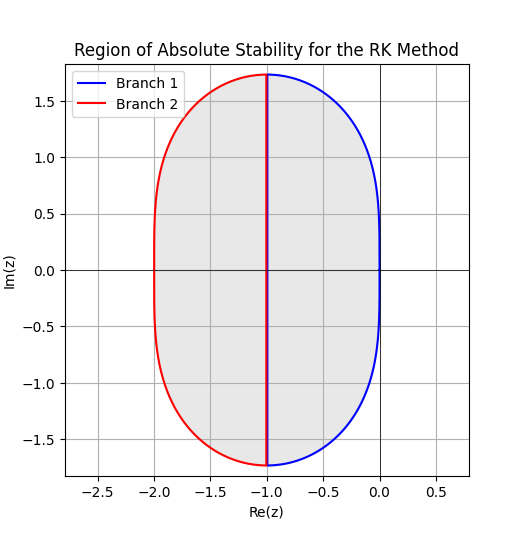
\includegraphics[width=0.6\textwidth]{Q1.png}
    \caption{Region of absolute stability for the given Runge-Kutta method.}
\end{figure}

\noindent From the plot, we see that the region of absolute stability includes part of the left half-plane, but does not include the entire left half-plane. Therefore, the method is not A-stable and therefore not L-stable. However, since the method is a Runge-Kutta method, it is zero-stable. \\



\begin{problem} \\
    \textbf{Stability of the TR-BDF2 method (3 points).} The TR-BDF2 method is an implicit 2-stage Runge-Kutta method based on taking a half time step with the trapezoidal rule and then a half step with the 2-step BDF method:
    \begin{align*}
        U^{*} &= U^n + \frac{k}{4}\left( f(U^n) + f(U^{*}) \right), \\
        3U^{n+1} - 4U^{*} + U^n &= k f(U^{n+1}).
    \end{align*}
    \begin{enumerate}[(a)]
        \item Show that this method is second-order accurate using Taylor series expansions.
        \item Determine the region of absolute stability and plot it. Based on this, show that the method is L-stable.
    \end{enumerate}
\end{problem}







\begin{problem} \\ 
    \textbf{Stability of the midpoint method (5 points).} A minor variation on the trapezoidal method is the midpoint method: 
    \[
        U^{n+1} = U^n + k f\left( \frac{U^n + U^{n+1}}{2}, t_n + \frac{k}{2} \right).
    \]
    For constant-coefficient ODEs, this is exactly the same as the trapezoidal method.
    \begin{enumerate}[(a)]
        \item Show that this method is second-order accurate using Taylor series expansions.
        \item Show that this method is A-stable.
        \item Show that even if $\lambda$ varies in time, so that 
        \[
            u' = \lambda(t) u,
        \]
        an analogue of A-stability still holds, i.e., using the midpoint method,
        \[
            |U^{n+1}| \leq |U^n| \quad \text{if} \quad \text{Re}(\lambda(t)) \leq 0 %\quad \text{for all } t.
        \]
        This property is called AN-stability.
        \item Show that the trapezoidal method, on the other hand, is not AN-stable.
    \end{enumerate}
\end{problem}




\begin{problem} \\
    \textbf{The pizza problem (10 points).} The image below shows a map of the seventh floor of Van Vleck Hall. All the doors are open.
    \begin{center}
        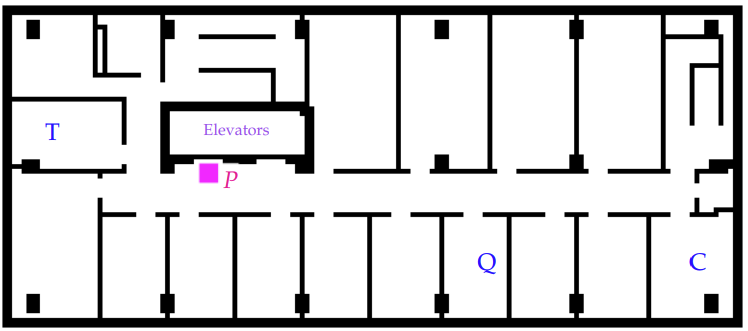
\includegraphics[width=0.8\textwidth]{Q4ProblemStatement.png}
        %\caption{Map of the seventh floor of Van Vleck Hall.}
    \end{center}
    A text file called "van\_vleck.txt" is provided that encodes this map as a $73 \times 160$ matrix using $1$ s for walls and $0$ s for open space. Use the convention that $(i,j) =(0,0)$ is the top left of the matrix and $(i,j) = (72,159)$ is the bottom right of the matrix. The grid spacing is $h = 22.5$ cm.
    

    A student exits the elevator holding a delicious pizza with a strong smell,
        which covers the region $P$ over gridpoints $(i,j)$ with $36\le i < 40,
          44\le j <48$. Let $u(x,y,t)$ be the smell concentration of the pizza at time
        $t$ at position $\vx=(x,y)$. The concentration satisfies the diffusion
        equation
        \begin{equation}
          \frac{\p u}{\p t} = b \nabla^2 u
        \end{equation}
        where $b=0.55\,\text{m}^2\,\text{s}^{-1}$. In the region $P$ the field is
        kept fixed at $u(x,y)=1$. At each wall, the concentration satisfies a
        no-flux boundary condition,
        \begin{equation}
          \vec{n} \cdot \nabla u =0, \label{eq:wall_bc}
        \end{equation}
        where $\vec{n}$ is a unit vector normal to the wall.
        \begin{enumerate}[(a)]
          \item Write a program to solve for the smell concentration field inside
                the building, using the two-dimensional discretization
                \begin{equation}
                  \frac{u_{i,j}^{n+1} - u_{i,j}^n}{k} = b \frac{u_{i+1,j}^n + u_{i,j+1}^n - 4u_{i,j}^n + u_{i-1,j}^n+u_{i,j-1}^n}{h^2} \label{eq:2ddifffd}
                \end{equation}
                where \smash{$u_{i,j}^n$} is the numerical approximation of
                $u(jh,(72-i)h,nk)$. Choose the timestep to be \smash{$k =
                    \frac{h^2}{6b}$} or smaller. As initial conditions, use
                \begin{equation}
                  u_{i,j}^0=\begin{cases}
                    1 & \qquad \text{if $(i,j)\in P$,} \\
                    0 & \qquad \text{otherwise,}
                  \end{cases}
                \end{equation}
                and throughout the simulation, keep $u_{i,j}=1$ for $(i,j)\in P$.
                To account for the boundary condition in Eq.~\eqref{eq:wall_bc}, use the
                ghost node approach: when considering a point $(i,j)$ in
                Eq.~\eqref{eq:2ddifffd} that references an orthogonal neighbor $(i^*,j^*)$
                that is a wall, treat \smash{$u_{i^*,j^*}^n$} as equal to \smash{$u_{i,j}^n$}.
                As an example of this, suppose that at a particular $(i,j)$, the points
                $(i,j-1)$ and $(i+1,j)$ are within walls. Then, after taking into
                account the boundary conditions, the appropriate finite-difference
                relation is
                \begin{equation}
                  \frac{u_{i,j}^{n+1} - u_{i,j}^n}{k} = b \frac{u_{i,j+1}^n - 2u_{i,j}^n + u_{i-1,j}^n}{h^2} = 0. \label{eq:2ddiffrest}
                \end{equation}
                due to cancellation of some terms.
          \item Make two-dimensional plots of the scaled smell concentration field
                $[u(x,y)]^{1/4}$ at $t=1\,\text{s}, 5\,\text{s}, 25\,\text{s},
                  100\,\text{s}$. Here, the quarter power helps to enhance small smell
                concentrations for visualization purposes. In the program files, there
                are some example programs that you may find useful, which make plots of a
                two-dimensional field with the map overlaid. You should expect that your
                program may take a reasonable amount of wall-clock time, possibly up to
                ten minutes to simulate to $t=100\,\text{s}$. You may wish test your
                program over smaller intervals of $t$ and consider possible code
                optimizations if necessary.
        \end{enumerate}
\end{problem}


\begin{problem}[4 Continued] \\
    \begin{enumerate}
        \item[(c)] Three professors T, Q, and C are trying to work at locations $(31,14)$,
                $(58,103)$, and $(58,147)$, respectively. Calculate the time in seconds to one decimal
                place when each professor will be distracted by the pizza smell, defined as
                when $u$ first exceeds $10^{-4}$ at each location.
          \item[(d)] Make a semilog plot\footnote{For the initial times, the smell
                  concentration in your numerical results will likely be zero, so this will
                  not be visible on the semilog plot. However, it will become visible once
                  the smell reaches that location. A reasonable vertical range for the
                  semilog plot is $10^{-10} \le u \le 1$.} showing the smell concentration at
                the three professors' locations over the range $0 \le t \le 100\,\text{s}$.
    \end{enumerate}
\end{problem}



\end{document}